\documentclass[border=20pt]{standalone}
\renewcommand\familydefault{\sfdefault} % Default family: serif 
\usepackage[usenames,dvipsnames]{xcolor}
\usepackage{tikz}
\usepackage{soul}
\usetikzlibrary{calc} 
\usetikzlibrary{arrows, decorations.markings,positioning,backgrounds,shapes}
\definecolor{WIRE}{HTML}{002FA7} % Klein Blue
\usepackage{ulem}
\renewcommand{\ULdepth}{3pt}

\newcommand\whiteuline{\bgroup\markoverwith
	{\textcolor{white}{\rule[-0.5ex]{2pt}{0.4pt}}}\ULon}

\tikzset{FK/.style={thick,<-,thick,>=latex}}

\newbox\ubox
\begin{document}
	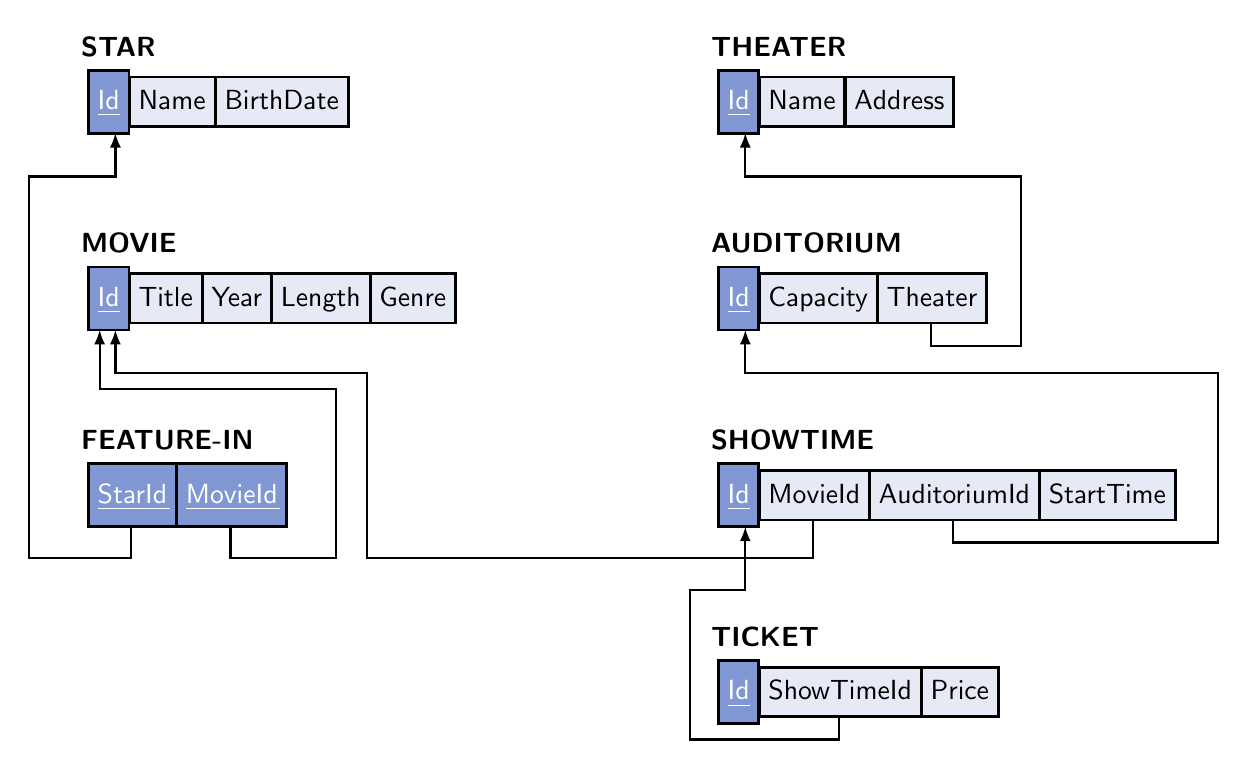
\begin{tikzpicture}[
	PK/.style={% Style for empatized boxes
		rectangle, line width =1pt,
		anchor=west,
		underline, % new property
		align=center,
        text=white,
		minimum height=.8cm,
		text height=1.5ex,
		text depth=.25ex,
        fill=WIRE!50,
		draw=black,
	},
	A/.style={% Style for normal boxes.
		rectangle, 
		line width =1pt,
		anchor=west,
		align=left,
		minimum height=.6cm,
		text height=1.5ex,
		text depth=.25ex,
        fill=WIRE!10,
		draw=black,
		inner ysep=5pt
	},
	underline/.append style={% define new style property
		execute at begin node={%
			\setbox\ubox=\hbox\bgroup
		},
		execute at end node={%
			\egroup\whiteuline{\box\ubox}%
		}
	},
	] % Uff that is all the configuration for tickzpicture xD
	
	% Define an brute force objet "Frame"
	% Variables 1:Position, 2: Identifier, 3: Title of frame 4: Subframe/Boxtype
	\def\Frame(#1)#2[#3]#4{%
		\begin{scope}[shift={(#1)}] 
		\node[font=\bf, anchor=west] (Title) at (-0.2,0.7) {#3}; 
		\edef\k{0}% Variable for box positión
		\edef\x{0}% Variable for named coordinate centering - below box
		\foreach \id/\style in {#4} {%enter sub frame data Name/Boxtype ,Name2/Boxtype | An space before Boxtype is needed 
			\node[\style] (h) at (\k pt,0) {\id}; %  % Draw a node depending on the variables.
			\pgfmathparse{\k+0.5*width{"\id"}+3.4pt} % Uses the textwidth to calculate named coordinate  
			\xdef\x{\pgfmathresult} % The resul is saved in the variable \x
			\draw (\x pt,-0.4) coordinate (\id#2); %Create a named coordinate concatenated: "sub frame data Name"+"identifier"
			\pgfmathparse{\k+width{"\id"}+6.8pt}% Calculate positión for each subframe box.       
			\xdef\k{\pgfmathresult}% Save the value to be added to the next iteration value.
		}    
		\end{scope}
	}% disadvantages: Is not posible to use Frame data Name like: Name_another_desc instead I use Name-another-desc


%STAR(Id (PK), Name, BirthDate)  
%MOVIE(Id (PK), Title, Year, Length, Genre)  
%FEATURE-IN(StarId (PK, FK to STAR.Id), MovieId (PK, FK to MOVIE.Id))  
%THEATER(Id (PK), Name, Address)  
%AUDITORIUM(Id (PK), Capacity, Theater (FK to THEATER.Id))  
%SHOWTIME(Id (PK), MovieId (FK to MOVIE.Id), AuditoriumId (FK to AUDITORIUM.Id), StartTime)  
%TICKETS(Id (PK), ShowTimeId (FK to SHOWTIME.Id), Price)  

\Frame(0,0){1}[STAR]{
	Id/PK,
	Name/A,
	BirthDate/A};

\Frame(0,-2.5){2}[MOVIE]{
	Id/PK,
	Title/A,
	Year/A,
	Length/A,
	Genre/A};

\Frame(0,-5){3}[FEATURE-IN]{
	StarId/PK,
	MovieId/PK};

\Frame(8,0){4}[THEATER]{
	Id/PK,
	Name/A,
	Address/A};

\Frame(8,-2.5){5}[AUDITORIUM]{
	Id/PK,
	Capacity/A,
	Theater/A};

\Frame(8,-5){6}[SHOWTIME]{
	Id/PK,
	MovieId/A,
	AuditoriumId/A,
	StartTime/A};


\Frame(8,-7.5){7}[TICKET]{
	Id/PK,
	ShowTimeId/A,
	Price/A};

\draw[FK] % From StarId3 to Id1
(Id1)++(0.1,0) -- ++(0,-.55) -- ++(-1.1,0) coordinate (inter)
-- (StarId3 -| inter) -- ++(0,-0.4) coordinate (inter)
-- (StarId3 |- inter) --++(0, 0.4);

\draw[FK] % From MovieId3 to Id2
(Id2)++(-0.1,0) -- ++(0,-.75) -- ++(3,0) coordinate (inter)
-- (MovieId3 -| inter) -- ++(0,-0.4) coordinate (inter)
-- (MovieId3 |- inter) --++(0,0.4);

\draw[FK] % From Theater5 to Id4
(Id4)++(0.1,0) -- ++(0,-.55) -- ++(3.5,0) coordinate (inter)
-- (Theater5 -| inter) -- ++(0,-0.2) coordinate (inter)
-- (Theater5 |- inter) --++(0,0.3);

\draw[FK] % From MovieId6 to Id2
(Id2)++(0.1,0) -- ++(0,-.55) -- ++(3.2,0) coordinate (inter)
-- (MovieId6 -| inter) -- ++(0,-0.4) coordinate (inter)
-- (MovieId6 |- inter) --++(0,0.5);

\draw[FK] % From AuditoriumId6 to Id5
(Id5)++(0.1,0) -- ++(0,-.55) -- ++(6,0) coordinate (inter)
-- (AuditoriumId6 -| inter) -- ++(0,-0.2) coordinate (inter)
-- (AuditoriumId6 |- inter) --++(0,0.3);


\draw[FK] % From ShowTimeId7 to Id6
(Id6)++(0.1,0) -- ++(0,-.8) -- ++(-.7,0) coordinate (inter)
-- (ShowTimeId7 -| inter) -- ++(0,-0.2) coordinate (inter)
-- (ShowTimeId7 |- inter) --++(0,0.3);

\end{tikzpicture}
\end{document}